% SENG3011 Testing Documentation
\title{Testing Report}
\author{Nicholas Grasevski \and Daniel Morton \and George El-Boustani \and Christopher Tin-Loi}
\date{\today}

\documentclass{article}
\usepackage{graphicx}

\begin{document}
\maketitle

% Teams must produce 1 document describing the testing processes used in the
% development of the product and attach their testing data.

\section{Architecture}
% The latest version of your architecture. Indicate which components are
% being tested and the type of testing (functional or non-functional)

\begin{figure}
\centering
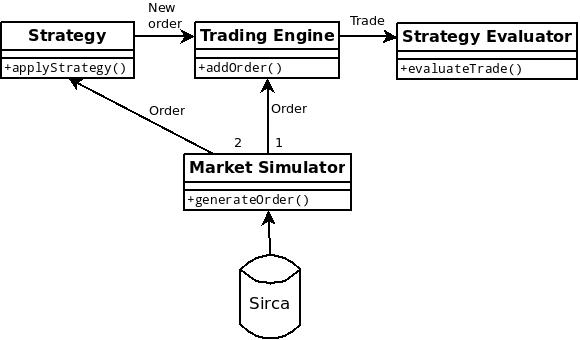
\includegraphics[width=0.8\textwidth]{architecture}
\caption{ATS Architecture Flowchart}
\label{fig:architecture}
\end{figure}

Our algorithmic trading system is essentially a function which takes a signal generator, an engine, a strategy evaluator and market data and outputs the evaluation, as well as the list of resultant trades. The user chooses and configures the appropriate plugins (signal generator, engine, strategy evaluator), chooses the input market data and then runs the simulation. The chosen strategy evaluator then outputs the evaluation to the user, and the list of trades is also outputted to the user.

We test our software at a variety of levels:
\begin{description}
  \item[Unit] At the lowest level we test our individual classes and functions, such as the plugins (signal generator, engine, strategy evaluator). We have various unit tests written for our software, following the naming convention ``module\_test.py", where ``module" is the name of the module being tested. We also have black box testing of components in the form of doctest strings, that is, example use cases embedded in the source code as comments, which can be run using Python's ``doctest". Our unit testing only checks against our functional requirements.
  \item[Integration] The combinations of various plugins are tested in a black box fashion by running the command line program with sample input and configuration parameters and the expected output is compared with the actual output. We have tests for both functional requirements (such as regression testing) and non-functional testing (such as load, performance, scalability, stress and volume testing).
  \item[System] The developers each have a test script which runs whenever they make a change to the software. This acts as a sanity check, protecting against developers from contributing if the program fails to work on their environment. It also alerts developers to changes made by others which break the system for them. This tests both our functional requirements (correctness) and non-functional requirements (compatibility).
  \item[Acceptance] We leave acceptance testing to the user, because this is suited to our Agile development process.
\end{description}

\section{Environment}
% Describe your testing environment: e.g. environment and/or tools used,
% limitations (e.g. things that are not tested)

% Software used during testing (if any)

Our testing relies on a range of POSIX tools and Python libraries which are available on most Unix distributions as well as Windows under MinGW or Cygwin:
\begin{description}
  \item[bash] We use the unix shell scripting language to tie all our tests together for batch test runs
  \item[diff] For black box testing, to see whether the expected output matches the actual output
  \item[time] For performance benchmarks
  \item[pep8] For syntax and style checking
  \item[pyflakes] Used for syntax and style checking
  \item[unittest] The standard Python unit testing framework
  \item[doctest] Verifies example use cases in the source code documentation
\end{description}

There are limitations to our testing:
\begin{description}
  \item[static type safety] Being a dynamically typed interpreted language, we have very few guarantees that our program matches our functional specification and instead we rely on test cases and syntax and style checking to find bugs.
  \item[property testing] We don't do any automated testing of the desired properties of our program and its components.
  \item[coverage] We did not check the coverage of our unit tests.
  \item[usability] We have no tests for usability of our system and instead leave it to the customer to evaluate the usability.
\end{description}

\section{Data}
% Overview of test data (test cases).

% Test input files (order files)
% Result files (if any)

\section{Process}
% Illustrate your testing process i.e. how your team conducts testing using
% the test data described earlier (e.g. in which order). How do you make sure
% you do not break old features when introducing new features?

% Test configuration files


\end{document}
